\documentclass[a4paper]{article}

\usepackage[english]{babel}
\usepackage[utf8]{inputenc}
\usepackage{amsmath}
\usepackage{graphicx}
\usepackage[colorinlistoftodos]{todonotes}
\usepackage{listings}
\usepackage{color}
\usepackage{csvsimple}
\usepackage{pgfplots}
\definecolor{mygreen}{rgb}{0,0.6,0}
\definecolor{mygray}{rgb}{0.5,0.5,0.5}
\definecolor{mymauve}{rgb}{0.58,0,0.82}

\lstset{ 
  backgroundcolor=\color{white},   % choose the background color; you must add \usepackage{color} or \usepackage{xcolor}; should come as last argument
  basicstyle=\footnotesize,        % the size of the fonts that are used for the code
  breakatwhitespace=false,         % sets if automatic breaks should only happen at whitespace
  breaklines=true,                 % sets automatic line breaking
  captionpos=b,                    % sets the caption-position to bottom
  commentstyle=\color{mygreen},    % comment style
  deletekeywords={...},            % if you want to delete keywords from the given language
  escapeinside={\%*}{*)},          % if you want to add LaTeX within your code
  extendedchars=true,              % lets you use non-ASCII characters; for 8-bits encodings only, does not work with UTF-8
  frame=single,	                   % adds a frame around the code
  keepspaces=true,                 % keeps spaces in text, useful for keeping indentation of code (possibly needs columns=flexible)
  keywordstyle=\color{blue},       % keyword style
  language=C++,                 % the language of the code
  morekeywords={*,...},            % if you want to add more keywords to the set
  rulecolor=\color{black},         % if not set, the frame-color may be changed on line-breaks within not-black text (e.g. comments (green here))
  showspaces=false,                % show spaces everywhere adding particular underscores; it overrides 'showstringspaces'
  showstringspaces=false,          % underline spaces within strings only
  showtabs=false,                  % show tabs within strings adding particular underscores
  stepnumber=2,                    % the step between two line-numbers. If it's 1, each line will be numbered
  stringstyle=\color{mymauve},     % string literal style
  tabsize=2,	                   % sets default tabsize to 2 spaces
  title=\lstname                   % show the filename of files included with \lstinputlisting; also try caption instead of title
}

\title{CS3210 Assignment 2 Report}

\author{Tan Xin You A0135812L}

\date{\today}

\begin{document}
\maketitle

\section{Implementation}
\label{sec:introduction}
\subsection{\texttt{ProofOfWorkGenerator} Class}
The main class that will calculate a valid digest from the parameters it was initialized with: \texttt{std::string prevDigest}, \texttt{std::string id}, \texttt{ulong target}.

Upon calling one of its \texttt{generate} function, \texttt{ProofOfWorkGenerator} calls \texttt{generateKernel} function to generate the valid digest. 

\subsection{\texttt{generateKernel} function}
\texttt{generateKernel}, as shown in Figure \ref{fig:generate-kernel}, uses the following arguments:

\begin{figure}
\begin{lstlisting}
__global__ void generateKernel(const uint8_t* templateX, ullong* nonce, uint8_t* digest, ulong target, bool* found)
\end{lstlisting}
\caption{\label{fig:generate-kernel} \texttt{generateKernel} function in \texttt{ProofOfWorkGenerator.cu}}
\end{figure}

\begin{description}
\item[{\texttt{templateX}}]A pointer to the template for the calculating a valid digest. Basically, from the 415\textsuperscript{th} bit to the 64\textsuperscript{th} bit of X, proof of work, as described in the assignment (see Figure \ref{fig:proof-of-work} for reference). This pointer is initialized with the \texttt{cudaMallocManaged} in the unified memory where any processor in the system can access, similar to defining a variable as a \texttt{\_\_managed\_\_}, allowing both device and host code to access this variable.
\begin{figure}
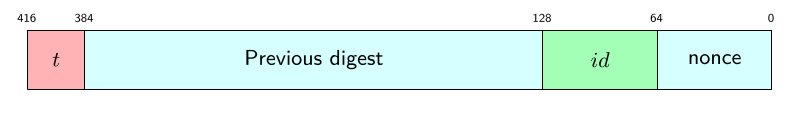
\includegraphics[width=1\textwidth]{Screenshot_3.png}
\caption{\label{fig:proof-of-work}Screenshot of proof of work from assignment.}
\end{figure}

\item[{\texttt{nonce}}]A pointer to another unified memory created by \texttt{cudaMallocManaged} where a valid nonce will be stored in when found. 

\item[{\texttt{digest}}]A \texttt{cudaMallocManaged} created pointer to an unified memory to store the digest of the proof-of-work with the stored \texttt{nonce}.

\item[{\texttt{target}}]The specified target, as described in the assignment.

\item[{\texttt{found}}]A \texttt{cudaMallocManaged} created pointer to an unified memory to store a boolean which indicates true when a valid nonce is found. A Cuda's \texttt{atomicCAS} function is used to check and toggle this value to prevent synchronization issues between threads, as shown in Figure \ref{fig:update-nonce}. This way only one thread is able to modify the memory for \texttt{nonce} and \texttt{digest} in each execution.
\end{description}

Each thread will execute \texttt{generateKernel} in these steps:
\begin{enumerate}
    \item Calculates the number of values to try as nonce.
    \item Calculates its own thread id, unique throughout the system.
    \item Copy \texttt{templateX} from the unified memory.
    \item Try the range of values iteratively until \texttt{found} is \texttt{true}
        \begin{enumerate}
            \item Calculate the hash using the given \texttt{sha256} function
            \item Verify if the first 64 bits of the hash is below \texttt{target}
            \item If below target, it is a valid nonce. Store the found nonce and set \texttt{found} to be \texttt{true}.
        \end{enumerate}
\end{enumerate}

\begin{figure}
\begin{lstlisting}
if(verified && !atomicCAS(found, false, verified))
{
    atomicExch(nonce, i);
    for(unsigned j=0; j<DIGEST_SIZE_IN_BYTES;++j)
    {
        digest[DIGEST_SIZE_IN_BYTES - j - 1] = hash[j];
    }
    return;
}
\end{lstlisting}
\caption{\label{fig:update-nonce} Update \texttt{nonce} code in \texttt{generateKernel} from \texttt{ProofOfWorkGenerator.cu}}
\end{figure}

\section{Assumptions}
\subsection{Given SHA256 code accepts proof-of-work in Big-Endian}
At least this is my understanding from what I read from the code. I used little-endian in my code mostly in the beginning as it was easier for me to code but realized later that the given \texttt{sha256} code uses big-endian. There wasn't much of an issue but the reader should not be shocked by the usage of little-endian in parts of the code.

\subsection{Max dimensionality of grid and block configuration}
I assumed 2D to be the maximum dimensionality to be used. I felt there is little use in using 3D configuration as my code does not require communication between threads, thus no need for complex configuration to aid communication.

\subsection{Using different epoch on every trial}
Due to the requirement, in order to compute a proof-of-work, the epoch used must be different on every trial. This creates more uncertainty in the experiments as some epoch may cause the proof-of-work to require a nonce lower in order of the range which a thread tries. However, we assume that running many enough trials per configuration would smoothen out this effect.

\section{Results}
\subsection{Experiment set up (for result reproduction)}
Experiments to get measurement were done on the compute cluster machines(xgpd0) and the jetson machine in the lab (jetsontx2-03). One can run \texttt{make benchmark} to run the same experiments. Input files used in the experiments are:
\begin{description}
    \item[{\texttt{1.in}}] As per the example in assignment. $target = 2^{48}$.
    \item[{\texttt{2.in}}] Same digest as \texttt{1.in}, $target = 2^{40}$.
    \item[{\texttt{3.in}}] Same digest as \texttt{1.in}, $target = 2^{32}$.
    \item[{\texttt{4.in}}] Digest: a6d569d489eca7f807e2edad9876473b918694ef68b5125585f5a9d667224033, $target = 2^{48}$
    \item[{\texttt{5.in}}] Same digest as \texttt{4.in}, $target = 2^{40}$
\end{description}

\begin{tikzpicture}
\begin{axis}
\addplot table [x={Num of Threads}, y={Avg Time Taken(s)}, col sep=comma, smooth] {xgpd.csv};
\end{axis}
\end{tikzpicture}

\begin{table}
    \centering
    \csvautotabular{xgpd.csv}
    \caption{\label{table:xgpd} Measurements taken from experiments ran on xgpd machine.}
\end{table}

\section{Modifications}
\subsection{Using busy wait instead of \texttt{CudaDeviceSynchronize}}
My initial design requires the CPU thread to wait for the termination of all threads via the use of \texxttt{CudaDeviceSynchronize}. I realize that this becomes counter-productive when I try to scale using more blocks and threads, see Figure \ref{fig:generateCudaDeviceSynchronize}. The \texttt{__host__} code will have to wait for more threads to terminate as it scales resulting in time wasted before the program outputs the result. I circumvent this by using a busy wait strategy in the \texttt{generateBusyWait}, see Figure \ref{fig:generateBusyWait}. The result is an average of 10-15% speedup in large enough grid and block configuration. One might think that the speedup shouldn't have been that significant, as most threads should immediatelly terminate when it \texttt{return} after reading \texttt{found} as \texttt{true}. However, when using big enough configuration, there is a lot of context switching involved when each new block runs, I suspect this is the reason for the significant speedup. Until Cuda develops a better way to terminate all running threads and/or stop them before they get run, this workaround seems to be the only way to avoid waiting for complete termination of the threads. However, resources will still be used for these threads' intialization, one can imagine a worse situation if the kernel function used requires more registers, or if each thread intialization involves more memory copying work.

\begin{figure}
\begin{lstlisting}
void ProofOfWorkGenerator::generateCudaDeviceSynchronize()
{
    dim3 gridDim(this->gridDimX, this->gridDimY);
    dim3 blockDim(this->blockDimX, this->blockDimY);

    generateKernel<<<gridDim, blockDim>>>(this->templateX, this->nonce, this->digest, this->target, this->found);
    cudaDeviceSynchronize();

    if(*(this->found) == 1)
    {
        cerr << "Found " << this->getNonce() << endl;
    } else 
    {
        cerr << "Failed\n";
    }
    check_cuda_errors();
}
\end{lstlisting}
\caption{\label{fig:generateCudaDeviceSynchronize} \texttt{generateCudaDeviceSynchronize} function in texttt{ProofOfWorkGenerator.cu}}
\end{figure}

\begin{figure}
\begin{lstlisting}
void ProofOfWorkGenerator::generateBusyWait()
{
    dim3 gridDim(this->gridDimX, this->gridDimY);
    dim3 blockDim(this->blockDimX, this->blockDimY);

    generateKernel<<<gridDim, blockDim>>>(this->templateX, this->nonce, this->digest, this->target, this->found);
    while(*(this->found) != 1);
    cerr << "Found " << this->getNonce() << endl;
    check_cuda_errors();
}
\end{lstlisting}
\caption{\label{fig:generateBusyWait} \texttt{generateBusyWait} function in texttt{ProofOfWorkGenerator.cu}}
\end{figure}

\end{document}
